\clearpage
\section{Corrected Poisson representation diagnostic}
\label{app:oracle-confirmation}

The nonzero-correction representation fits originally reported by the
Poisson lane remain retracted under amendment A10. A separate rerun on
the complete original development cohort now confirms the corrected
query-metric projection (job \provOracleConfirmationJob, scientific source
\texttt{\provOracleConfirmationSource}, retained evidence pinned at
\texttt{\provOracleConfirmationPin}). All
\nOracleConfirmationFits{} case/rank fits meet the recorded stationarity
criterion; the independent NumPy field and derivative audit passes
\nOracleConfirmationChecks{} checks. These are untimed, truth-informed
representation fits on already opened cases. The historical timed
results, their source pins and the original retraction are unchanged.

Let $R_G$ be the triangular factor of the evaluated bank in the query
mesh's field norm, and let $Q_q$ have orthonormal columns spanning
$R_G C_q$. Eliminating the free correction coefficients leaves
\begin{equation}
 r_q(z)=(I-Q_qQ_q^\top)(R_Gh_\theta(z)-T).
\end{equation}
Here $T$ is the reference field projected into these coordinates.
The original implementation omitted the required normalization of the
projector. The corrected finite best-found error is an upper bound on
the unknown global minimum, while the free-bank floor is a lower bound.
At $q=R$, direct free-coefficient projection attains that floor and
removes the redundant nonlinear head.

\begin{table}[h]
\centering
\small
\setlength{\tabcolsep}{3pt}
\caption{Separately confirmed Poisson representation errors (\%) on the
original development sources. Original starts use the unchanged
nearest-training-code multistart prescription with the repaired projector.
Best found additionally permits previously retained solved states and the
preceding rank's best fit as feasible starts. Median summarizes the
safeguarded errors. Original starts and best found report worst-case
errors; bank floor is the worst free-bank projection error.
Stationary counts cases satisfying the normalized-gradient rule, with
the direct endpoint stationary by construction. None is a new inference
timing or sealed-test result.}
\label{tab:oracle-confirmation}
\resizebox{\linewidth}{!}{\input{tables/TC_oracle_confirmation}}
\end{table}

\clearpage
\section{Three-dimensional development comparisons}
\label{app:campaign-development}

\textbf{Provisional evidence, excluded from the abstract and main claims.}
The following panels are audited development comparisons during an
ongoing tuning campaign. Their inputs were available for checkpoint or
configuration selection. These tables preserve the recorded development snapshot; later frozen
final evaluations are not included here. Independent-seed confirmation
and final evaluation must be distinguished from checkpoint selection. Failure to reach an accuracy
target is retained as a result, and a finite training budget does not
establish a model family's attainable error floor. No cross-PDE or
cross-allocation runtime ratio is formed.

Each table pairs accuracy with the cost of the same solver invocation.
GPU warm-up precedes measurement, parameters use double precision and
matrix multiplications use the highest-precision setting. Query costs
include the recorded initialization, solve and requested field output
with inputs and outputs resident on the GPU; unmeasured host transfers
are not assigned a cost. Timing summaries retain all repetitions.
Operator variants include any stated interpolation or incompressibility
projection in the measured query. Failed direct mesh-transfer variants
are displayed separately from native-grid prediction followed by
interpolation; their failure is not an intrinsic impossibility result
for the operator family.

Stationarity columns report each run's recorded stopping criterion;
they do not prove a global minimum. The selected Poisson panel has
independently audited fields and references, but its nonlinear stopping
summary lacks saved selected latent states for a separate gradient
reconstruction. The selected Navier--Stokes panel retains histories for
sampled independent weak-gradient checks. Its new paired measurements
pass the numerical-validity audit, but a separate strict cross-run
frozen-field replay gate failed and remains failed. This supports neither
cross-run equivalence nor an implementation-speed ratio. A zero recorded
stopping-failure count does not remove these qualifications.

The weak NM-ROM residual is projected against smooth test functions.
The learned bank, compressed head and correction rank have sizes
$R$, $K$ and $q$; $M$ is the actual number of weak tests. The Burgers
basis completes the degenerate Laplacian eigenvalue shell at its
requested cutoff, preserving coordinate symmetry. Dense full-grid
operations remain charged where quadrature has not met its certificate.
Full-bank Galerkin controls and a full-bank weak least-squares endpoint
are distinct reduced equations. On the native grid, POD uses the matched
training states. On finer heat and Poisson meshes, POD is rebuilt offline
from the same training members; these mesh-adapted controls are distinct
from transferring frozen neural weights.
Efficient classical controls remain in the comparison even when they
are both faster and more accurate.

\begin{table}[h]
\centering
\caption{Provisional development panel provenance. Each row names a
separate GPU allocation. Scientific source identifiers refer to staged
file contents verified against repository history; snapshot hashes and
upstream result/audit hashes are in \texttt{tables/campaign-provenance.json}.}
\label{tab:campaign-sources}
\resizebox{\linewidth}{!}{% Generated by gen_campaign_supplement.py; do not edit.
\begin{tabular}{lllll}
\toprule
PDE & Attempt & Job & GPU & Scientific source \\
\midrule
Burgers 3D & b3d004 & 3995688 & A100 80GB PCIe & \texttt{c026d56b8390} \\
Heat 3D & extra03 & 3995709 & A100-PCIE-40GB & \texttt{4ac8b16455f5} \\
Poisson 3D & extra03 & 3995104 & A100 80GB PCIe & \texttt{a50ce0977373} \\
Navier--Stokes 3D & extra03 & 3995695 & A100 80GB PCIe & \texttt{8ba0a11ee83a} \\
\bottomrule
\end{tabular}
}
\end{table}

\begin{table}[h]
\centering
\caption{Provisional training and query contracts from saved run
configurations. Grid counts are per spatial axis. Fields are full spatial states, including the initial
state when requested; vector states include all channels. The number
of fields is not a count of statistically independent examples. Heads
lists saved trained candidates; the following panels explicitly identify
the displayed candidate. All model families share the lane's training
membership.}
\label{tab:campaign-setup}
\resizebox{\linewidth}{!}{% Generated by gen_campaign_supplement.py; do not edit.
\begin{tabular}{llrrrrrrr}
\toprule
PDE & Training grid & Train cases & Fields/case & Outputs & Channels & $R$ & $K$ & $M$ \\
\midrule
Burgers 3D & 33 nodes & 512 & 8 & 51 & 1 & 256 & 32 & 642 \\
Heat 3D & 32 intervals & 128 & 6 & 6 & 1 & 128 & 8, 16, 32 & 512 \\
Poisson 3D & 32 intervals & 512 & 1 & 1 & 1 & 128 & 8, 16 & 512 \\
Navier--Stokes 3D & 32 periodic points & 512 & 6 & 6 & 3 & 512 & 16 & 1024 \\
\bottomrule
\end{tabular}
}
\end{table}

\clearpage
\begin{table}[h]
\centering
\caption{Provisional operator training records. Budget, done and selected
are requested, completed and checkpoint-selected optimizer updates;
batch is examples per update and LR is the initial learning rate.
Seed records the initializer. Exit records why training stopped.
Selection uses the recorded development criterion; an update limit is
not a convergence certificate. Reused training checkpoints may originate
in an earlier allocation. Compute budgets are recorded, not claimed equal.}
\label{tab:campaign-training}
\resizebox{\linewidth}{!}{% Generated by gen_campaign_supplement.py; do not edit.
\begin{tabular}{llrrrrrrrl}
\toprule
PDE & Operator & Parameters & Budget & Done & Selected & Batch & LR & Seed & Exit \\
\midrule
Burgers 3D & fno & 1771431 & 20000 & 20000 & 16100 & 2 & 0.001 & 920310 & steps \\
Burgers 3D & unet & 89431 & 20000 & 20000 & 17500 & 2 & 0.001 & 920311 & steps \\
Burgers 3D & deeponet & 1861959 & 30000 & 30000 & 30000 & 2 & 0.001 & 920312 & steps \\
Burgers 3D & transolver & 564392 & 30000 & 30000 & 29400 & 2 & 0.001 & 920313 & steps \\
Heat 3D & fno\_w16\_m6 & 1771349 & 20000 & 20000 & 19500 & 4 & 0.001 & 920321 & steps \\
Heat 3D & unet\_w8 & 89197 & 20000 & 20000 & 20000 & 4 & 0.001 & 920322 & steps \\
Heat 3D & deeponet\_r128\_w16 & 857749 & 20000 & 20000 & 20000 & 4 & 0.001 & 920323 & steps \\
Heat 3D & transolver\_w48\_s32 & 562840 & 20000 & 20000 & 20000 & 4 & 0.001 & 920324 & steps \\
Poisson 3D & fno\_w24\_m8 & 9440953 & 30000 & 30000 & 26750 & 2 & 0.0005 & 920450 & steps \\
Poisson 3D & unet\_w16 & 354577 & 30000 & 30000 & 28750 & 2 & 0.0005 & 920451 & steps \\
Poisson 3D & deeponet\_r128\_w16 & 791697 & 30000 & 30000 & 29000 & 2 & 0.001 & 920452 & steps \\
Poisson 3D & transolver\_w48\_s32 & 561272 & 30000 & 30000 & 29750 & 2 & 0.001 & 920453 & steps \\
Navier--Stokes 3D & deeponet & 6790319 & 32000 & 32000 & 23200 & 2 & 0.001 & 202609208 & steps \\
Navier--Stokes 3D & transolver & 569064 & 32000 & 32000 & 32000 & 2 & 0.001 & 202609209 & steps \\
Navier--Stokes 3D & fno & 4196511 & 8000 & 8000 & 7100 & 2 & 0.001 & 202609205 & steps \\
Navier--Stokes 3D & unet & 89287 & 8000 & 8000 & 7900 & 2 & 0.001 & 202609206 & steps \\
\bottomrule
\end{tabular}
}
\end{table}

FNO is a Fourier neural operator; U-Net is a multiscale convolutional
model; DeepONet uses an input branch and coordinate trunk; Transolver
uses learned physics-attention slices. The pinned machine-readable
training records retain each architecture, normalization, selected
checkpoint hash and training curve metadata. Burgers operators return
their trained time knots, pass through the supplied initial state and
interpolate to the common requested output times. The Navier--Stokes
case is a periodic interacting three-component flow family; the
reported panel does not claim turbulent-flow coverage. Each selected
panel now includes paired measurements for all four operator families.

\clearpage
\begin{table}[h]
\centering
\caption{Provisional NM-ROM architecture and training records, derived
from saved checkpoints and their original training metadata. MLP widths
list input, hidden and output sizes of each multilayer perceptron. Head
parameter counts include its linear skip; optimized training codes and
fixed Fourier, scale and whitening assets are excluded. Budget, done
and selected are requested, completed and checkpoint-selected updates.
Base seed initializes the recipe; stage-specific key splits and sampling
seeds are retained in the pinned configuration. Selected updates follow
the recorded development criterion or the final optimizer iterate, as
specified in the machine-readable protocol. Update limits do not
certify convergence. Reused checkpoints retain their original training
record rather than inheriting the query allocation's budget.}
\label{tab:campaign-nmrom-training}
\resizebox{\linewidth}{!}{% Generated by gen_campaign_supplement.py; do not edit.
\begin{tabular}{lllrrrrr}
\toprule
PDE & Part & MLP widths & Parameters & Budget & Done & Selected & Base seed \\
\midrule
Burgers 3D & bank & $128\!\to\!384\!\to\!384\!\to\!256$ & 295936 & 200000 & 200000 & 200000 & 920201 \\
Burgers 3D & head K32 & $32\!\to\!256\!\to\!256\!\to\!256$ & 148224 & 100000 & 100000 & 100000 & 920201 \\
Heat 3D & bank & $64\!\to\!256\!\to\!256\!\to\!128$ & 115328 & 100000 & 100000 & 100000 & 920312 \\
Heat 3D & head K8 & $8\!\to\!256\!\to\!256\!\to\!128$ & 102016 & 80000 & 80000 & 80000 & 920312 \\
Heat 3D & head K16 & $16\!\to\!256\!\to\!256\!\to\!128$ & 105088 & 80000 & 80000 & 80000 & 920312 \\
Heat 3D & head K32 & $32\!\to\!256\!\to\!256\!\to\!128$ & 111232 & 80000 & 80000 & 45000 & 920312 \\
Poisson 3D & bank & $128\!\to\!256\!\to\!256\!\to\!128$ & 131712 & 150000 & 150000 & 150000 & 920412 \\
Poisson 3D & head K8 & $8\!\to\!256\!\to\!256\!\to\!128$ & 102016 & 100000 & 100000 & 100000 & 920412 \\
Poisson 3D & head K16 & $16\!\to\!256\!\to\!256\!\to\!128$ & 105088 & 100000 & 100000 & 100000 & 920412 \\
Navier--Stokes 3D & bank & $512\!\to\!512\!\to\!512\!\to\!1536$ & 1313280 & 12000 & 12000 & 12000 & 202609204 \\
Navier--Stokes 3D & head K16 & $16\!\to\!512\!\to\!512\!\to\!512$ & 542208 & 30000 & 30000 & 30000 & 202609204 \\
\bottomrule
\end{tabular}
}
\end{table}

The coordinate network supplies the spatial bank, which is frozen while
the compressed coefficient head is trained. The head's optimized
training codes are offline fitting variables, not an encoder or online
inputs. The vector bank's output groups all velocity components;
its terminal width therefore differs from the number of bank functions.
Correction directions and query-mesh solver assets are prepared offline.
Changing correction rank within a reported ladder leaves all neural
weights frozen. The pinned protocol records checkpoint content hashes,
full training configurations and the source of reused training metadata.

\clearpage
\subsection{Burgers 3D: provisional development panel}
\label{app:campaign:0}
\textbf{Provisional:} Audited development data with all four operator families and the same training membership. Errors use the initial-field norm and exclude time zero. Operator predictions interpolate trained time knots to the common output times. The newer operator schedules are still under evaluation. Physical refinement covers only two cases; this panel supports same-grid comparisons only.\par
\begin{table}[h]
\centering
\small
\setlength{\tabcolsep}{3pt}
\caption{33 nodes per axis; 8 development cases per method. Initial-field-normalized evolved error; same-grid reference. Each accuracy/cost pair comes from the same invocation in job 3995688. NF/NS counts nonfinite/nonstationary cases; outliers count calls above $1.5$ times the method median.}
\label{tab:campaign:0}
\resizebox{\linewidth}{!}{\input{tables/TC_development_0}}
\end{table}
\FloatBarrier
\noindent All timed arms in the main panel are included. The separately measured larger-head candidate on the same allocation is retained in the complete report, alongside representation and limited refinement diagnostics. FOM labels identify nonlinear (n) and inner linear (l) tolerances.\par
\begin{figure}[h]
\centering
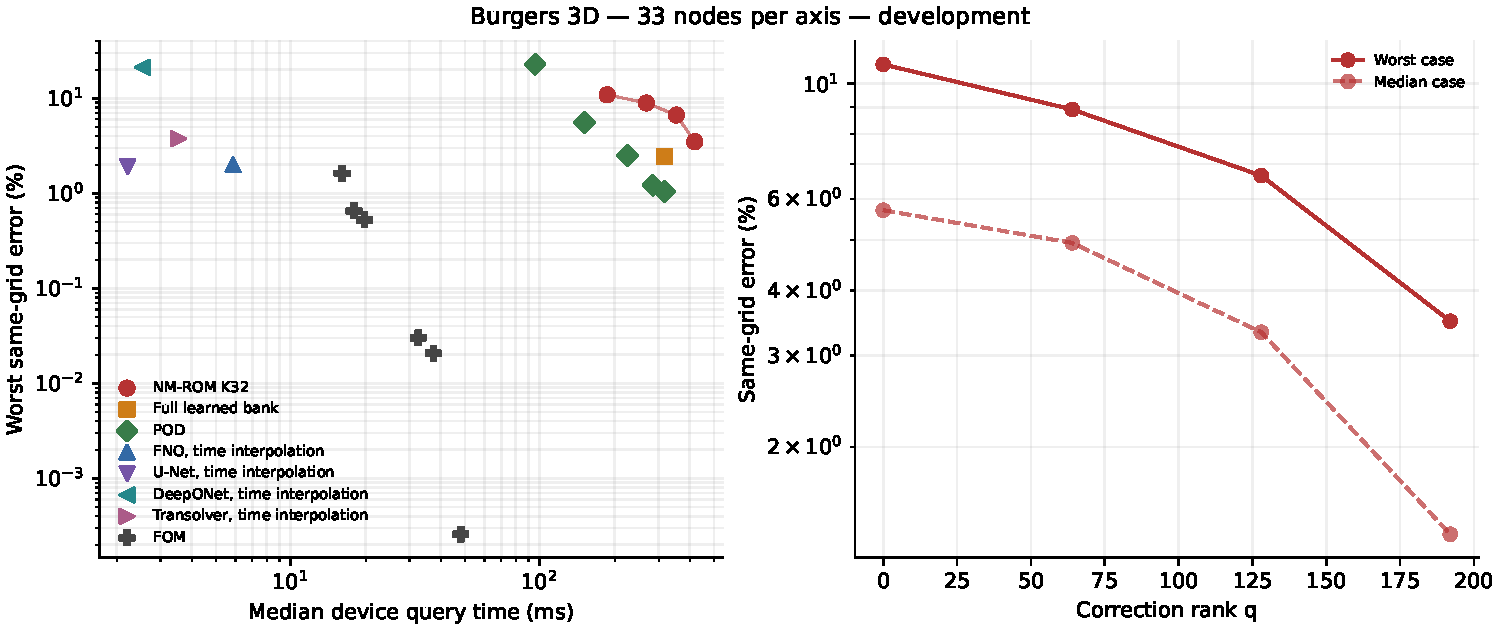
\includegraphics[width=\linewidth]{evidence/campaign-2026-09-20/burgers3d-b3d004-n33.pdf}
\caption{Provisional paired development measurements from Table~\ref{tab:campaign:0}. The right panel isolates the fixed-head correction ladder; the left retains classical controls and operator variants. Zero-error direct solves are identified separately rather than clipped onto the logarithmic error axis.}
\label{fig:campaign:0}
\end{figure}
\clearpage
\subsection{Heat 3D: provisional development panel}
\label{app:campaign:1}
\textbf{Provisional:} Audited development data with all four operator families. Errors use the current reference-field norm and exclude time zero. All recorded fits and evolved solves are stationary. The larger head improves the high-correction endpoint but retains a generalization gap; improved initialization and longer operator schedules are under evaluation. Failed direct transfer variants are retained; native-grid interpolation is charged separately. Finer-grid POD is rebuilt offline from the same training members; it is a mesh-adapted classical control, not frozen-weight transfer.\par
\begin{table}[h]
\centering
\small
\setlength{\tabcolsep}{3pt}
\caption{64 intervals per axis; 16 development cases per method. Current-reference-normalized evolved error; same-grid reference. Each accuracy/cost pair comes from the same invocation in job 3995709. NF/NS counts nonfinite/nonstationary cases; outliers count calls above $1.5$ times the method median.}
\label{tab:campaign:1}
\resizebox{\linewidth}{!}{\input{tables/TC_development_1}}
\end{table}
\FloatBarrier
\noindent The complete audited report retains smaller-head ladders, intermediate POD ranks and time-step diagnostics. Failed sampled-quadrature certificates remain in the earlier attempt and are not promoted.\par
\begin{figure}[h]
\centering
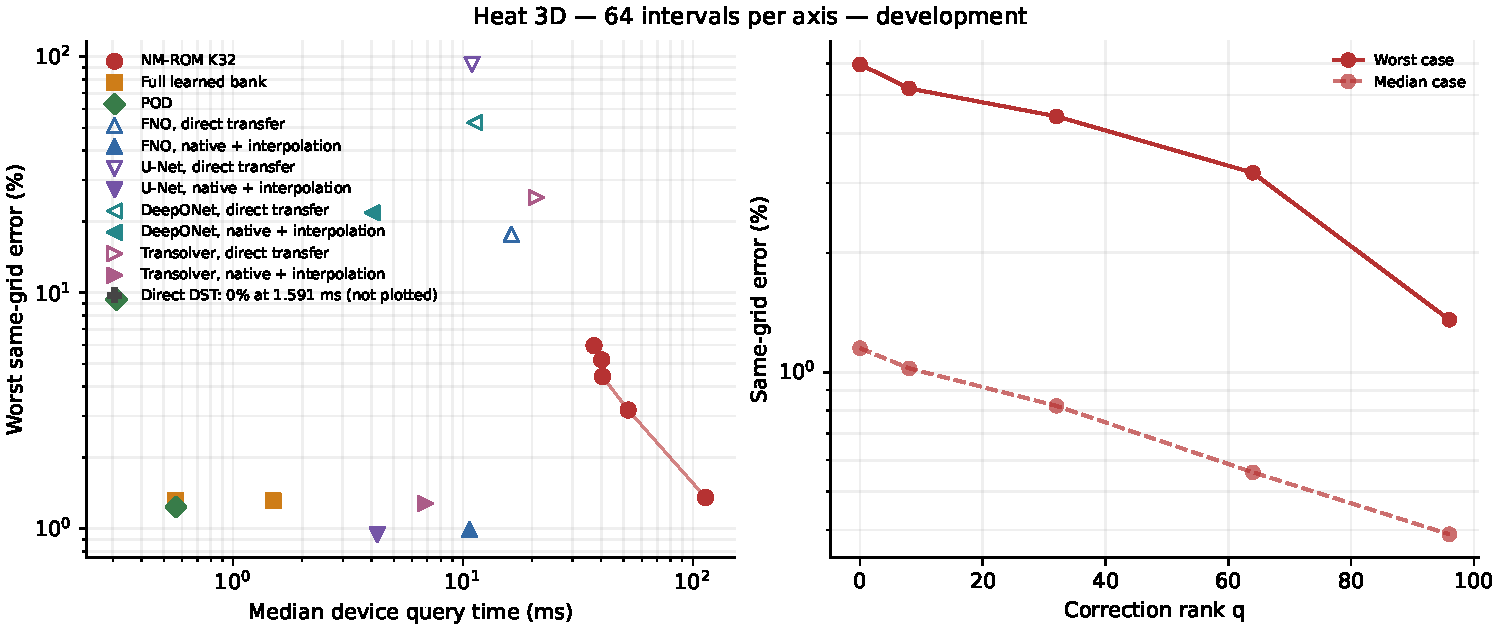
\includegraphics[width=\linewidth]{evidence/campaign-2026-09-20/heat3d-extra03-n64.pdf}
\caption{Provisional paired development measurements from Table~\ref{tab:campaign:1}. The right panel isolates the fixed-head correction ladder; the left retains classical controls and operator variants. Zero-error direct solves are identified separately rather than clipped onto the logarithmic error axis.}
\label{fig:campaign:1}
\end{figure}
\clearpage
\subsection{Poisson 3D: provisional development panel}
\label{app:campaign:2}
\textbf{Provisional:} Audited development data with all four operator families. Static weights are placed on the GPU during setup. New operator curves are still improving and longer common schedules are under evaluation. Direct transfer variants and quadrature certificates fail; preserved-domain FNO padding is a pending control. Every measured pair below shares one allocation. Finer-grid POD is rebuilt offline from the same training members; it is a mesh-adapted classical control, not frozen-weight transfer. The saved stopping records are internally consistent, but selected latent states were not retained for an independent weak-gradient audit.\par
\begin{table}[h]
\centering
\small
\setlength{\tabcolsep}{3pt}
\caption{64 intervals per axis; 16 development cases per method. Relative field error against the same-grid discrete solution. Each accuracy/cost pair comes from the same invocation in job 3995104. NF/NS counts nonfinite/nonstationary cases; outliers count calls above $1.5$ times the method median.}
\label{tab:campaign:2}
\resizebox{\linewidth}{!}{\input{tables/TC_development_2}}
\end{table}
\FloatBarrier
\noindent The complete audited report retains the K8 ladder, intermediate POD ranks, and failed sampled-quadrature diagnostics. They are not presented as missing experiments.\par
\begin{figure}[h]
\centering
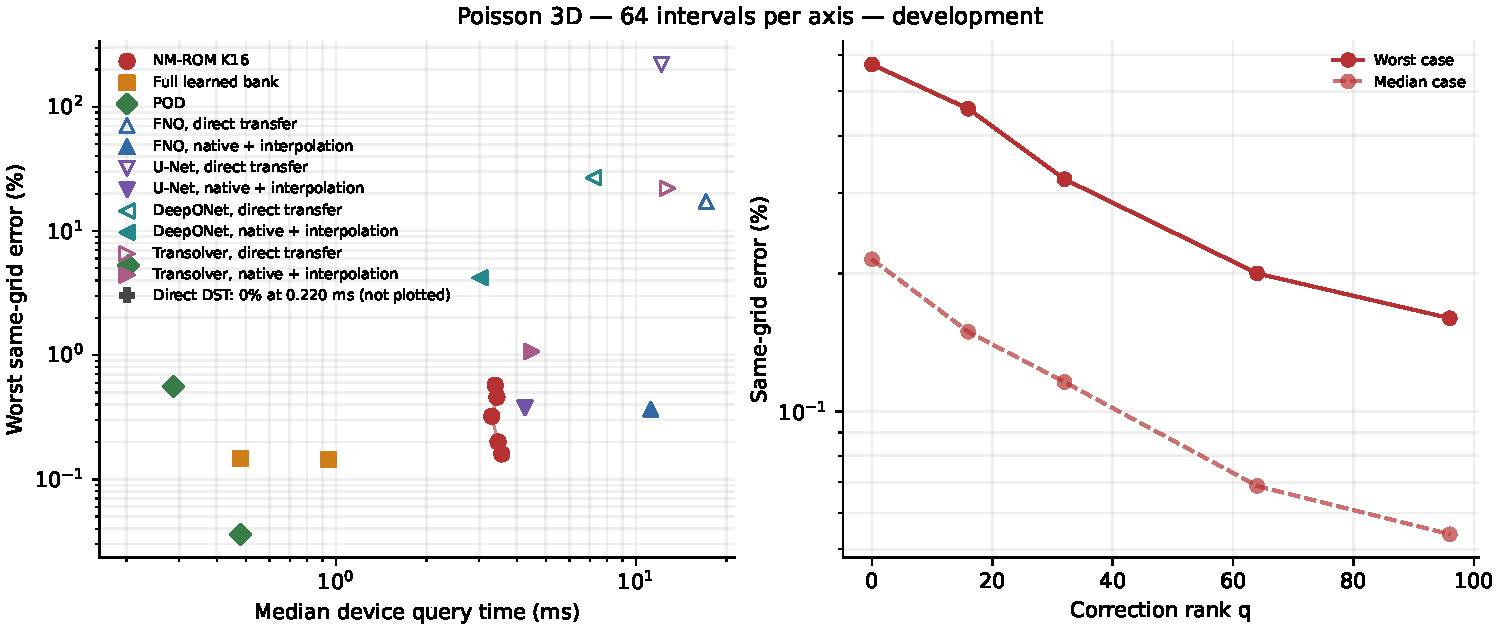
\includegraphics[width=\linewidth]{evidence/campaign-2026-09-20/poisson3d-extra03-n64.pdf}
\caption{Provisional paired development measurements from Table~\ref{tab:campaign:2}. The right panel isolates the fixed-head correction ladder; the left retains classical controls and operator variants. Zero-error direct solves are identified separately rather than clipped onto the logarithmic error axis.}
\label{fig:campaign:2}
\end{figure}
\clearpage
\subsection{Navier--Stokes 3D: provisional development panel}
\label{app:campaign:3}
\textbf{Provisional:} Independently audited new paired development measurements with all four operator families. Errors use the initial vector-field norm and exclude time zero. Learned-bank and head accuracy targets fail. Saved latent histories support sampled independent weak-gradient checks. A strict cross-run frozen-field replay gate failed and remains failed; no numerical-equivalence or implementation-speed claim is made. Augmented training and larger-bank tuning remain in progress.\par
\begin{table}[h]
\centering
\small
\setlength{\tabcolsep}{3pt}
\caption{32 periodic points per axis; 8 development cases per method. Initial-field-normalized evolved error; same-grid reference. Each accuracy/cost pair comes from the same invocation in job 3995695. NF/NS counts nonfinite/nonstationary cases; outliers count calls above $1.5$ times the method median.}
\label{tab:campaign:3}
\resizebox{\linewidth}{!}{\input{tables/TC_development_3}}
\end{table}
\FloatBarrier
\noindent All timed arms are included; the separate larger-bank snapshot-fit diagnostics remain in the complete archive. Leray projection enforces discrete incompressibility and its online cost is charged.\par
\begin{figure}[h]
\centering
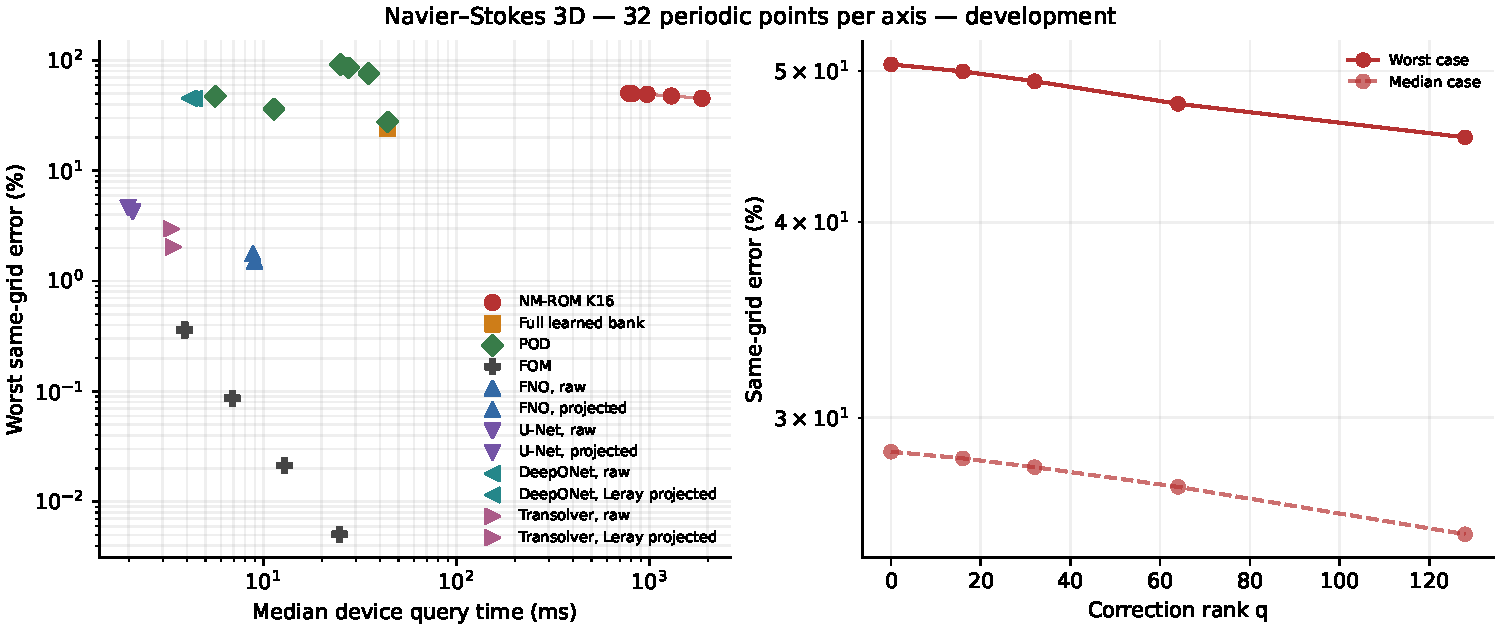
\includegraphics[width=\linewidth]{evidence/campaign-2026-09-20/ns3d-extra03-n32.pdf}
\caption{Provisional paired development measurements from Table~\ref{tab:campaign:3}. The right panel isolates the fixed-head correction ladder; the left retains classical controls and operator variants. Zero-error direct solves are identified separately rather than clipped onto the logarithmic error axis.}
\label{fig:campaign:3}
\end{figure}


\FloatBarrier
